% -*- coding: utf-8 -*-

\documentclass[14pt,xcolor={rgb}]{beamer}

\usetheme{gauss}

% remove these two lines to hide footlines in (sub)section pages
\setbeamertemplate{at begin section}[normal]
\setbeamertemplate{at begin subsection}[normal]

\usepackage[spanish]{babel}
\usepackage{arev}
\usepackage{multicol} %For writing text in columns
\setlength{\columnsep}{1cm} %Defines separation of columns
\usepackage{tcolorbox} % for text colorboxes

% For adding links
\usepackage{hyperref}
%\urlstyle{
%    colorlinks=true,
%    linkcolor=blue,
%    filecolor=magenta,      
%    urlcolor=cyan,
%    pdftitle={Overleaf Example},
%    pdfpagemode=FullScreen,
%    }
%\urlstyle{same}

\begin{document}

\title{Registro multimodal de im\'agenes mediante Informaci\'on Mutua}
\author{Bruno M. Breggia}
\date{29 de Abril 2022}
\institute{FI-UNER}

\begin{frame}[plain]
\titlepage
\end{frame}

\begin{frame}{Paper Original}

{\tiny IEEE TRANSACTIONS ON MEDICAL IMAGING, VOL. 16, NO. 2, APRIL 1997.}

	\begin{center}
	``\textit{Multimodality Image Registration by Maximization of Mutual Information}"
	
	{\small Frederik Maes, Andr\'e Collignon, Dirk Vandermeulen, Guy Marchal, Paul Suetens}
	\end{center}

{\small Miembros del \textit{Laboratory for Medical Imaging Research}, Leuven, B\'elgica.}
\end{frame}

\section{Introducci\'on}

\begin{frame}{El Problema}
\textbf{Registro de im\'agenes}: proceso de transformaci\'on de diferentes conjuntos de datos (im\'agenes) a un mismo sistema coordenado.
\begin{center}
	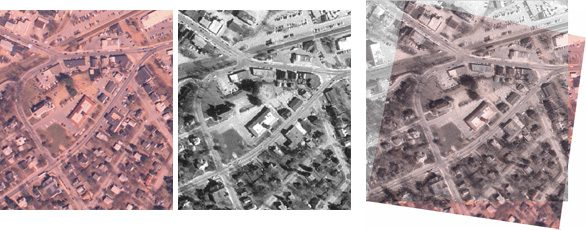
\includegraphics[scale=0.5]{Images/registration.jpg}
\end{center}
\end{frame}

\begin{frame}{Aplicaci\'on}

Visi\'on computacional, imagenolog\'ia m\'edica, reconocimiento autom\'atico de blancos militares, astrofotograf\'ia.

\begin{center}
	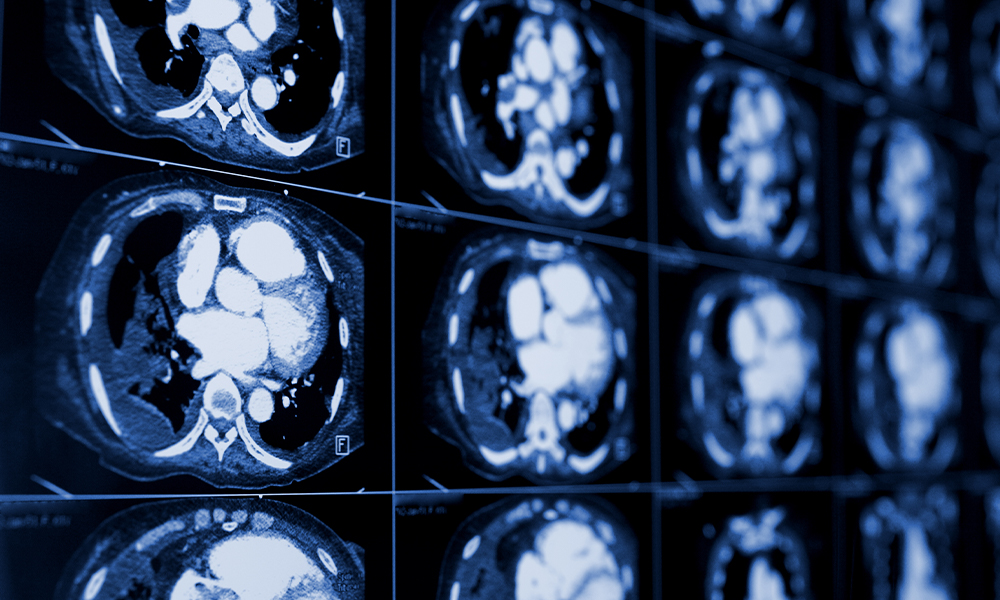
\includegraphics[scale=0.2]{Images/medical_imaging.jpg}
\end{center}
\end{frame}

\begin{frame}{Aplicaci\'on: Imagenolog\'ia M\'edica}
% Registro multimodal de im\'agenes m\'edicas
\begin{center}
	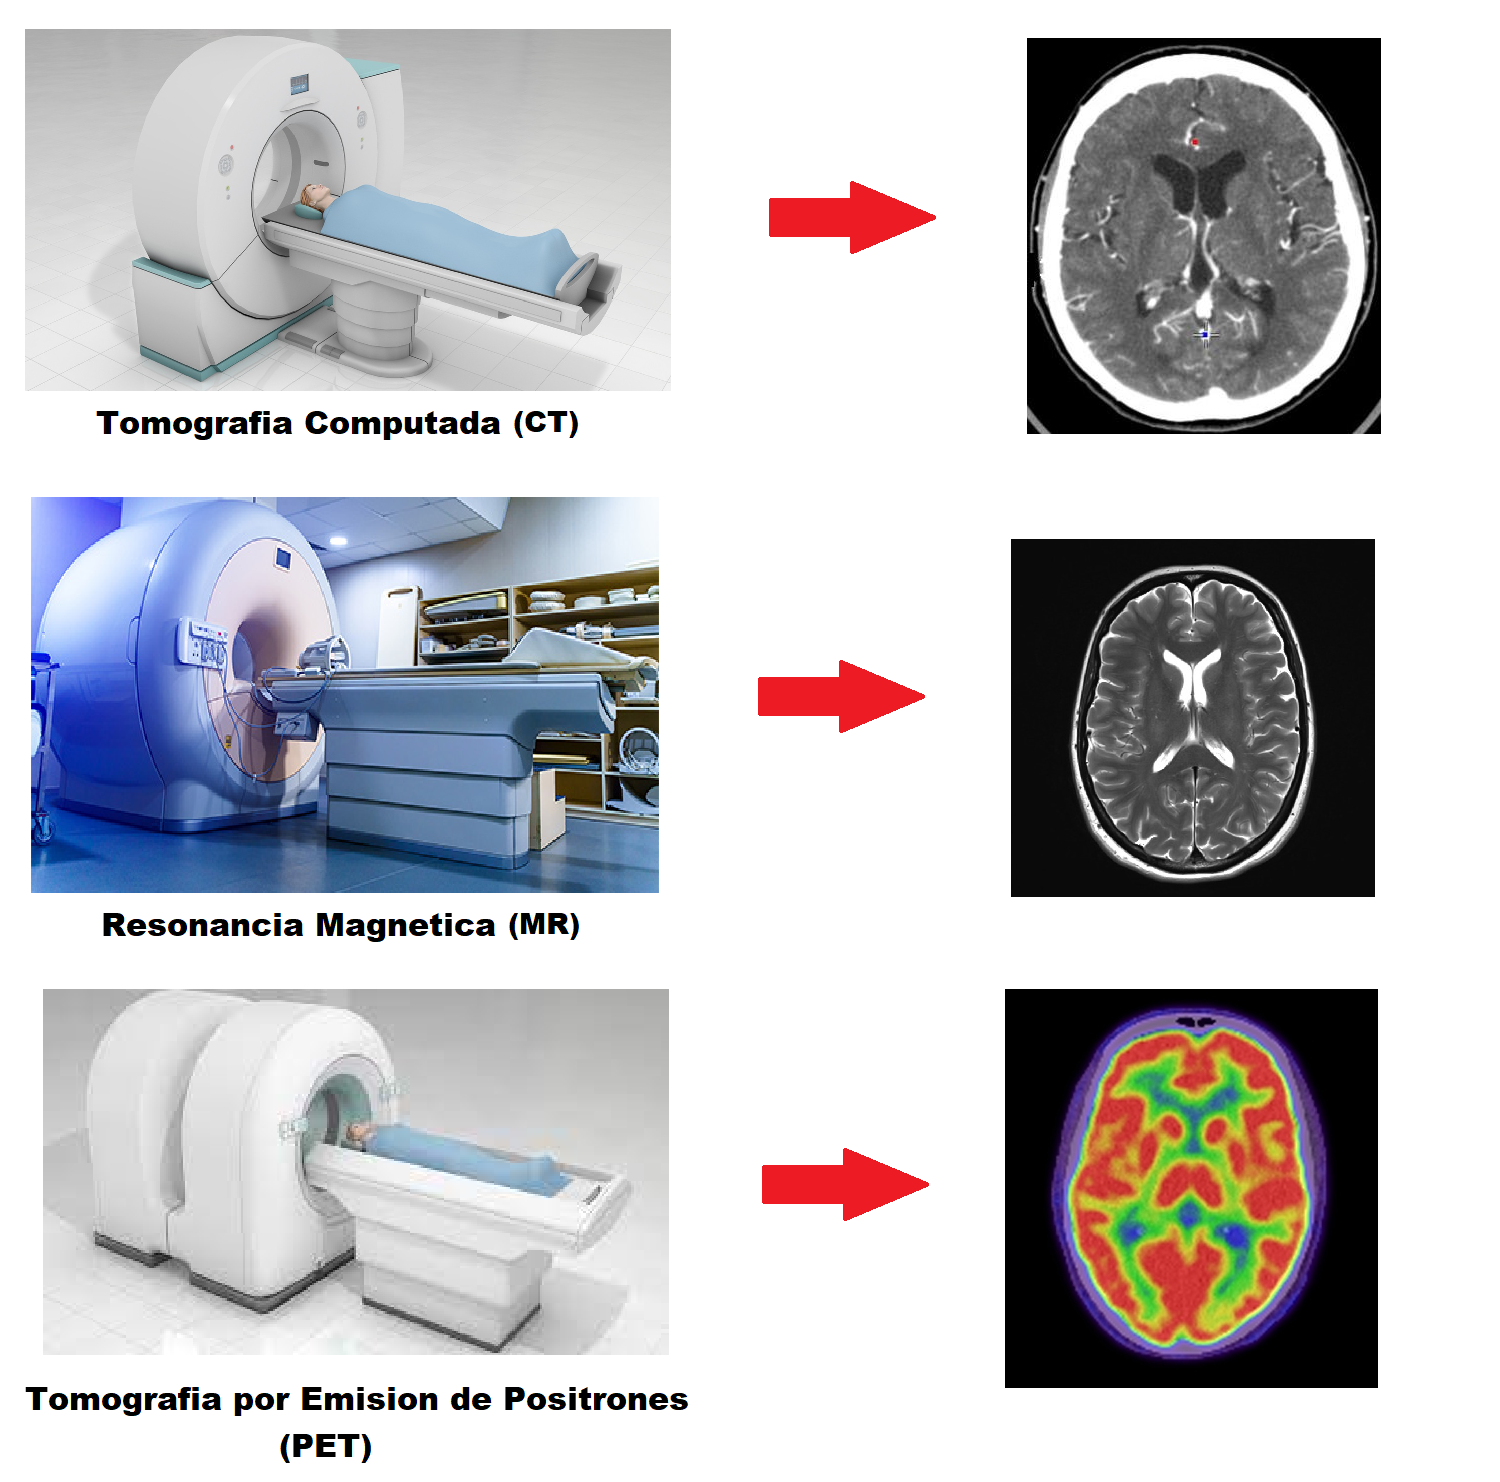
\includegraphics[scale=0.18]{Images/multimodality.png}
\end{center}
\end{frame}

\begin{frame}{T\'ecnicas convencionales}
\small
\begin{multicols} {2}
Los m\'etodos habituales para el registro de im\'agenes son:
\begin{enumerate}
	\item[$\bullet$] Basado en \textit{frames} (estereot\'actico)
	\item[$\bullet$] Basado en puntos caracter\'isticos de la imagen
	\item[$\bullet$] Basado en superficies
	\item[$\bullet$] Basado en v\'oxeles
\end{enumerate}
\begin{center}
	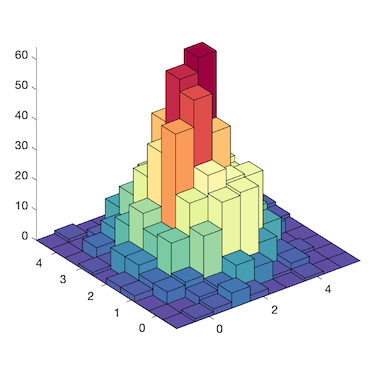
\includegraphics[scale=0.5]{Images/hist2d.png}
	Histograma 2D
\end{center}
\end{multicols}
\end{frame}

\section{Un Nuevo Criterio de Registro}

\begin{frame}{Informaci\'on Mutua}
\footnotesize Informaci\'on Mutua (o Entrop\'ia Relativa) es un par\'ametro que cuantifica el grado de dependencia de dos variables aleatorias A y B a partir de la similitud entre la probabilidad conjunta $p_{AB}$ con el producto de las marginales $p_Ap_B$.

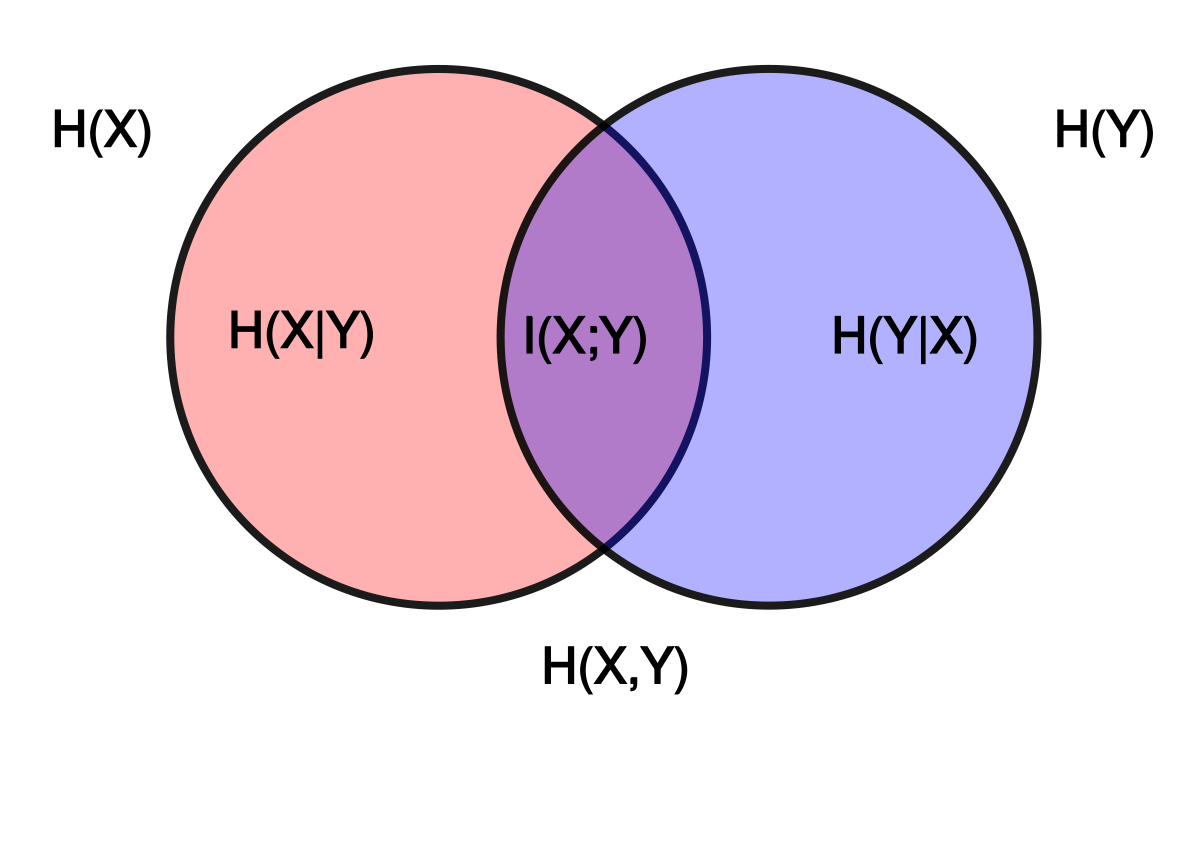
\includegraphics[scale=0.15]{Images/mutual-information-diagram.png}
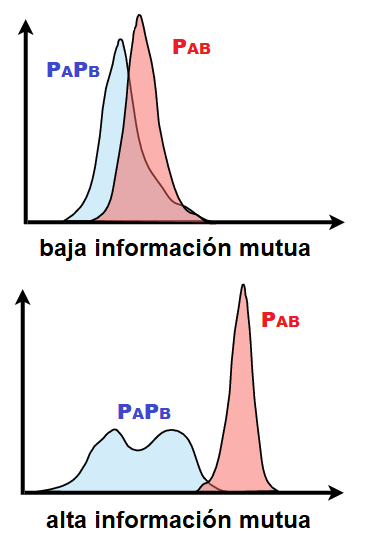
\includegraphics[scale=0.35]{Images/pdf_distance.png}
\end{frame}

\begin{frame}{Propiedades de Informaci\'on Mutua}
% Frame \insertframenumber
\small
\begin{itemize}
	\item[$\bullet$] No negativa
	$$I(A,B)\geq 0$$
	\item[$\bullet$] Independencia
	$$I(A,B)=0 \iff p_{AB}(a,b)=p_A(a)p_B(b)$$
	\item[$\bullet$] Simetr\'ia $$I(A,B)=I(B,A)$$
	\item[$\bullet$] Informaci\'on propia $$I(A,A)=H(A)$$
\end{itemize}
\end{frame}


\begin{frame}{Procedimiento 1}
\small
Se toman dos im\'agenes, una ser\'a la \textbf{imagen de referencia (R)} y la otra la \textbf{imagen flotante (F)}, que iremos desplazando y rotando.

La transformaci\'on que nos permite ir de $F$ hasta $R$ es una transformaci\'on de cuerpo r\'igido (traslaciones y rotaciones).

\begin{center}
	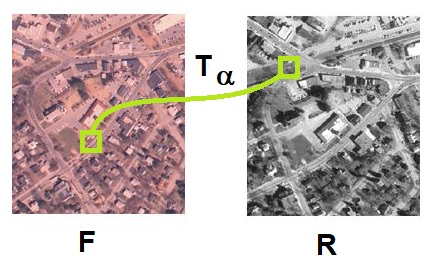
\includegraphics[scale=0.5]{Images/transformacion.jpg}
\end{center}

%Si $s$ es el vector posici\'on para un voxel en $F$, dada las traslaciones $t_x, t_y, t_z$ y las rotaciones $\phi_x, \phi_y, \phi_z$, la posici\'on correspondiente en $R$ est\'a dada por el producto $sT_{\alpha}$, con $T_{\alpha}$ la matriz de transformaci\'on.

\end{frame}

\begin{frame}{Procedimiento 2}
\small
A partir de la transformaci\'on $T_{\alpha}$, se obtienen las intensidades de cada voxel de $F$ y la correspondiente de $R$. La frecuencia de ocurrencia de este par de valores permite armar un histograma 2D.
\begin{multicols} {2}
	\begin{eqnarray*}
	p_{FR,\alpha}(f,r) = \frac{h_{\alpha}(f,r)}{\sum\limits_{f,r}h_{\alpha}(f,r)}\\
	p_{F,\alpha}(f) = \sum\limits_r p_{FR,\alpha}(f,r)\\
	p_{R,\alpha}(r) = \sum\limits_f p_{FR,\alpha}(f,r)
	\end{eqnarray*}
	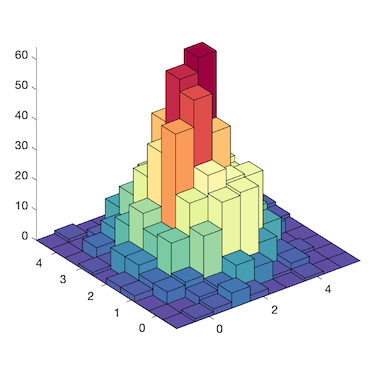
\includegraphics[scale=0.4]{Images/hist2d.png}
\end{multicols}
\end{frame}

\begin{frame}{Procedimiento 3}
\small
\begin{tcolorbox}[colback=green!5,colframe=green!40!black,title=Suposici\'on]
La dependencia estad\'istica entre las intensidades de los voxeles correspondientes de ambas im\'agenes es m\'axima si est\'an alineadas.
\end{tcolorbox}
$$I(\alpha) = \sum\limits_{f,r}p_{FR,\alpha}(f,r)\log \frac{p_{FR,\alpha}(f,r)}{p_{F,\alpha}(f)p_{R,\alpha}(r)}$$
La optimizaci\'on de la MI en base a las traslaciones y rotaciones se realiza num\'ericamente con el {\color{blue} \href{https://github.com/BrunoBreggia/Optimization_algorithms}{m\'etodo de Powell}}.
\end{frame}


\begin{frame}{Puesta a prueba 1}
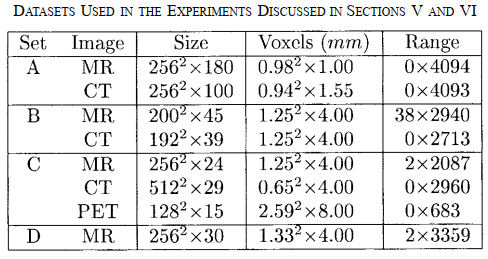
\includegraphics[scale=.80]{Images/dataset.png}
\end{frame}

\begin{frame}{Puesta a prueba 2}
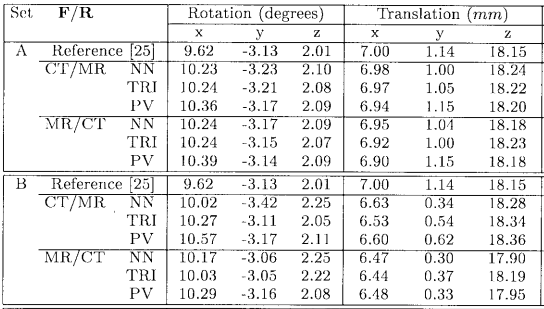
\includegraphics[scale=.75]{Images/resultados(1).png}
\end{frame}

\begin{frame}{Puesta a prueba 3}
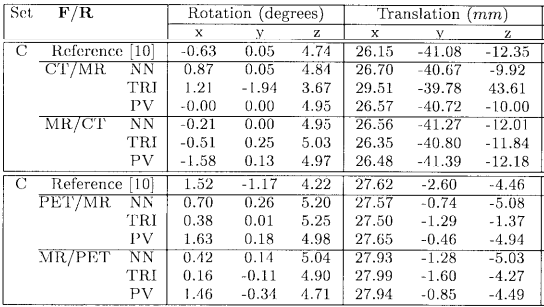
\includegraphics[scale=.75]{Images/resultados(2).png}
\end{frame}

\section{Discusi\'on y Conclusiones}

\begin{frame}{Discusi\'on y conclusiones}
\footnotesize
\begin{itemize}
	\item[$\bullet$] Este m\'etodo puede detectar relaciones no lineales entre las intensidades de im\'agenes multimodales.
	\item[$\bullet$] Permite detecci\'on de similitudes en base a criterios m\'as generales (no s\'olo transformaci\'on de cuerpo s\'olido).
	\item[$\bullet$] La selecci\'on de rasgos a comparar m\'as eficientes es un \'area a explorar.
	\item[$\bullet$] El proceso no es necesariamente igual de eficiente intercambiando $F$ con $R$, se desconoce el motivo.
	\item[$\bullet$] La variaci\'on continua y suave de la MI puede ser aprovechada con optimizaci\'on basada en gradientes.
	\item[$\bullet$] El proceso es directo: no requiere preprocesamiento ni interacci\'on con el usuario. Ideal para el \'ambito cl\'inico.
\end{itemize}
\end{frame}

\end{document}
